\documentclass[11pt,a4paper]{article}
\usepackage[T1]{fontenc}
\usepackage[margin=1in]{geometry}
\usepackage{amsmath,amssymb,mathtools}
\usepackage{booktabs}
\usepackage{graphicx}
\usepackage{xcolor}
\usepackage[colorlinks=true,linkcolor=blue!60!black,citecolor=blue!60!black,urlcolor=blue!60!black]{hyperref}
\usepackage{microtype}
\usepackage{xurl}
\setlength{\emergencystretch}{3em}
\usepackage{enumitem}
\usepackage[most]{tcolorbox}
\newtcolorbox{keybox}[1][]{colback=blue!3,colframe=blue!45!black,boxrule=0.5pt,left=4pt,right=4pt,top=3pt,bottom=3pt,#1}
\newtcolorbox{failbox}[1][]{colback=red!3,colframe=red!45!black,boxrule=0.5pt,left=4pt,right=4pt,top=3pt,bottom=3pt,#1}
\hypersetup{pdftitle={Gated exciton fluids II},pdfauthor={Xavier Callens},pdfsubject={Machine-checked kernel theorem, harmonic crystallisation estimate, edge energies, validity gate, exponential integrator}}

\begin{document}
\begin{center}
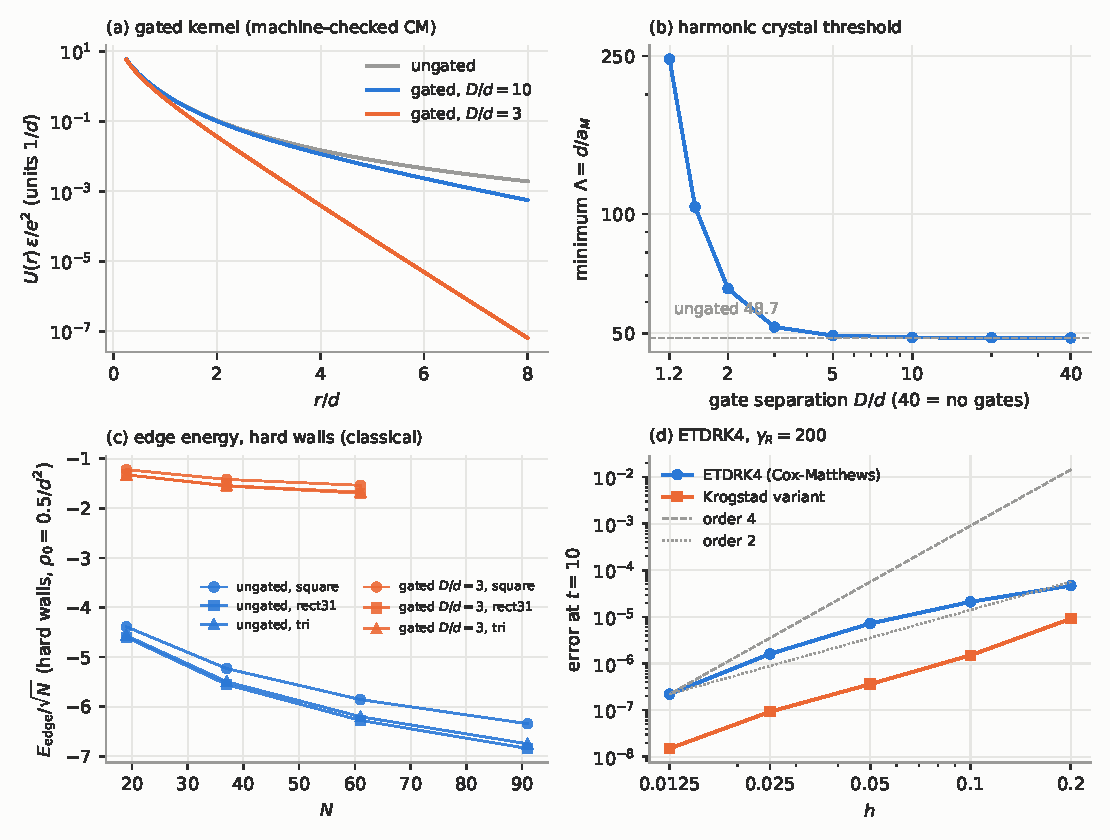
\includegraphics[width=0.97\textwidth]{figs_companion/fig_cover.pdf}\\[2pt]
{\footnotesize (a) Gated dipole kernel for two gate separations against the ungated kernel (Poisson series, $d=1$).
(b) Smallest $\Lambda=d/a_M$ admitting a harmonic-stable crystal against $D/d$ (eight sampled values; 40 stands for no gates).
(c) Edge energy per $\sqrt N$ of hard-wall containers, best configurations. (d) Error of ETDRK4 and of Krogstad's variant at the
registered stiffness against step size; guide lines are anchored at the smallest step.}
\end{center}
\vspace{-0.8em}
\begin{center}
{\Large\textbf{Gated exciton fluids II:}\\[2pt]
\large a machine-checked kernel theorem, a harmonic crystallisation estimate, open-boundary energies,\\ a validity gate for materials-data inputs, and an exponential integrator that did not meet its gate}\\[8pt]
Xavier Callens\\ {\small SocrateAI Research \quad\url{https://github.com/xaviercallens/SocrateAI-Scientific-QuantumFluids}}\\[2pt]
{\small October 2026}
\end{center}
\vspace{-0.4em}

\begin{abstract}\small\noindent
The first gated-exciton paper~\cite{CallensGated} proved on paper that grounded metal gates keep the dipolar exciton kernel
completely monotone (CM) in $r^2$, ran a pre-registered driven-dissipative solver test, and listed what was not done. This second paper
reports five of the follow-up packages. The four numerical packages (harmonic estimate, edge study, HF gate, ETD) carry a
pre-registration committed before their registered runs (with the exceptions disclosed in Section~\ref{sec:status}); the Lean package
has none. Each was read by an independent verifier before this deposit. \textbf{(1)}~The theorem is formalised in Lean~4/Mathlib: 52 theorems, no \texttt{sorry}, only the standard three axioms,
with the Poisson summation \emph{derived} (not assumed) and the Laplace density shown non-negative and bounded; the verifier compiled it
independently and recomputed the kernel by a direct image sum.
\textbf{(2)}~A harmonic Lindemann estimate of the crystallisation threshold, calibrated on a quantum-Monte-Carlo control, is a
\emph{negative} result for devices with $d\sim1$~nm: $d/a_M\gtrsim 49$ would be needed in a rigid-exciton model, gates raise
it at every sampled gate separation, and two registered predictions on the control failed or were refuted (one of them depends on a
definition in the QMC source that was not checked).
\textbf{(3)}~An open-boundary study of 65 classical $N$-particle configurations of three CM kernels finds a negative edge energy that
depends monotonically on the aspect ratio (with one disclosed exception), and no clean boundary law.
\textbf{(4)}~A Hugging Face / neural-network validity gate \emph{fails} for the two quantities the model needs.
\textbf{(5)}~An ETDRK4 integrator fails its registered order-4 gate on the stiff reservoir (consistent with stiff-order reduction), took 7.7\,s against 227\,s
for dense BDF to a stationary state on one seed, $8\times8$ grid, on a loaded machine, and has a step limit lower than the IMEX module's at high density.
Two packages, a matrix-free Newton--Krylov solver at $64\times64$ and a classical L6 node-arrangement design study, were still
running at deposit time and are \emph{not} reported and no verdict on them is implied. Written by an AI system; reviewed by independent instances; not refereed.
\end{abstract}

\section{Status, scope, and what was and was not verified}\label{sec:status}

\begin{keybox}
\textbf{Dependency.} The lattice theorem of Cohn--Kumar type used throughout~\cite{OpenAI2026,CohnKumar2007} is unrefereed and
AI-generated; every statement that uses it is conditional. Nothing here compares with experimental data.
\textbf{Process.} Each numerical package was run by a worker instance with a pre-registration committed before the registered runs
(dates and hashes in the repository), then re-checked by a fresh \emph{hostile verifier} that recomputed key numbers with its own code.
Exceptions: the Lean package has no pre-registration; in the HF package the one candidate data file was opened before the registration
(disclosed there); the Wigner registration has amendment A2, written after the scan and marked exploratory; the edge study's later
amendments are discussed in Section~\ref{sec:edge}.
Verifier verdicts: Lean \emph{accept}; Wigner, edge, HF gate, ETD \emph{accept with fixes}. The fixes are applied or disclosed below;
claims the verifier could not reproduce were dropped.
\end{keybox}

Where a number appears, it is copied from a committed result file (named in Section~\ref{sec:repro}); the figures are generated by
\texttt{exploration/exciton/python/companion\_figures.py} from those files. The only values typed into a figure script are the ETD
work--precision rows, copied from the ETD results note and marked as such in the script.

\section{Lean formalisation of the gated-kernel theorem}\label{sec:lean}

\textbf{Statement.} For grounded planes at $z=h_1$ and $z=-h_2$ ($P=2(h_1+h_2)$), an electron at $z_e$ and a hole at $z_h$ (any real
values), the image series of $V_{ee}+V_{hh}-2V_{eh}$ equals the Laplace transform $\int_0^\infty e^{-ts}\mu(s)\,ds$ of
$\mu(s)=(\pi s)^{-1/2}S(s)$ with $S(s)\ge 0$; hence the kernel is CM in $t=r^2$.

\textbf{What is proved} (file \texttt{exploration/exciton/lean/GatedKernel.lean}, 1083 lines, 52 theorems, built against Mathlib
v4.34.1; all 17 \texttt{\#print axioms} show \texttt{[propext, Classical.choice, Quot.sound]}):

\begin{center}\small
\begin{tabular}{@{}p{0.07\textwidth}p{0.85\textwidth}@{}}
\toprule
tier & content \\ \midrule
T1 & the trigonometric core $2-\cos2a-\cos2b-2\cos(b-a)+2\cos(a+b)=2(1-\cos(b-a))(1+\cos(a+b))=2(\sin a-\sin b)^2\ge0$; the image
offsets on each plane are a bijective re-indexing of the direct ones, so the lattice Green function vanishes on both planes \\
T2 & Poisson summation \emph{derived} from Mathlib's Gaussian/Jacobi-theta results for every real shift; $S_m\ge0$; $S(s)\ge0$ for all
$s>0$, all $h_1+h_2>0$, all real $z_e,z_h$ \\
T3 & $\mu$ is measurable, continuous and bounded on $(0,\infty)$; the Laplace transform is smooth with $(-1)^rg^{(r)}\ge0$ for all $r$
(a verbatim copy of the library's \texttt{AdmissiblePotential}); the series $\sum_n$ of image terms equals $\int e^{-ts}\mu(s)ds$ for every $t>0$ \\
\bottomrule
\end{tabular}
\end{center}

No theorem takes the Poisson identity, a summability fact or a measure-theoretic statement as a hypothesis; the only side conditions
are $0<s,t$ and $0<h_1+h_2$. The verifier compiled the file (exit 0, no warnings), found no \texttt{sorry}/\texttt{axiom}/
\texttt{native\_decide}, checked that the statement matches $V_{ee}+V_{hh}-2V_{eh}$ with the stated image positions, and
recomputed the kernel with its own three-dimensional image sum ($N=4000$): agreement with the Lean-side expression to $10^{-9}$ at three
radii and with the Laplace integral to $10^{-12}$.

\textbf{What it does not do.} It does not prove that 0 is excluded (the zero function is admissible), does not prove uniqueness of the
Green function, and does \emph{not} prove the lattice-optimality theorem of~\cite{OpenAI2026}: the Lean file shows the \emph{hypothesis}
of that theorem is met by the gated kernel, which is as far as the dependency goes. The layered-dielectric extension (a
Sturm--Liouville expansion) remains a remark, not part of this file.

\section{A harmonic estimate of the crystallisation threshold}\label{sec:wigner}

\textbf{Question.} At what exciton density does a dual-gated bilayer crystallise? A quantum-Monte-Carlo (QMC) answer needs a code and
compute that were not used; this package produces a \emph{harmonic Lindemann estimate} with a calibration error attached, not a
critical density. Literature gate (arXiv texts read by the worker and re-read by the verifier): the bare $1/r^3$ gas--solid transition
$n r_0^2=290(30)$ with Lindemann ratio $\gamma=0.230(6)$ (DMC)~\cite{Astrakharchik2007}, $n r_0^2\approx324$ (196--484, PIMC at
$T=0.014D/a^3$)~\cite{Buechler2007}; composite excitons with a crystal confined to a finite density window~\cite{Boening2011}; gated
Coulomb electrons where the harmonic and DMC critical gate distances are 35 and 29 (20\%)~\cite{Valenti2025}.
Dimensionless set-up: $\Lambda=r_0/d=d/a_M$, $\nu=nd^2$, $n r_0^2=\nu\Lambda^2$, $D=2h$.

\textbf{Pre-registered checks and outcomes.}
\begin{center}\small
\begin{tabular}{@{}p{0.31\textwidth}p{0.6\textwidth}@{}}
\toprule
item & result \\ \midrule
P0 lattice code vs.\ $E_{\triangle}/N=4.446(nr_0^2)^{3/2}$ & $4.4464$, deviation $8\times10^{-5}$: pass \\
P0 Laplace kernel vs.\ image series & relative difference $\le2.4\times10^{-8}$: pass \\
P1 harmonic ratio below the DMC one & \textbf{refuted}: $\gamma_h(290)=0.263$ vs.\ DMC $0.230(6)$ \\
P2 criterion A usable (ratio in $[0.5,2]$) & \textbf{failed}: $n_c^h=847$ (690--1047), ratio $2.9$ \\
P4 gates raise the threshold & confirmed \\
P4 monotone in $\nu$ & \textbf{refuted} for all bilayer kernels: interior minimum (the $2/x$ core); monotone only for pure $1/r^3$ \\
\bottomrule
\end{tabular}
\end{center}

\textbf{Calibrated estimate.} The harmonic Lindemann ratio follows $\gamma_h=c\,(nr_0^2)^{-1/8}$ with $c=0.5342$; the verifier
reproduced $c=0.534241$ with its own real-space image series and Brillouin-zone sum. Because $n_c\propto\gamma_c^{-8}$ the criterion is
extremely steep ($\gamma_c=0.25\to435$, $0.20\to2600$, $0.15\to2.6\times10^{4}$), so the generic ``$\gamma_c=0.1$--$0.2$'' is useless
here. Calibrating on the QMC control (criterion B, $\gamma_c=\gamma_h(290)=0.263$) gives, with a 20\% transfer error in the
controlling quantity assumed from~\cite{Valenti2025}:

\begin{itemize}[leftmargin=1.2em,itemsep=1pt]
\item \textbf{A rigid-exciton crystal needs a large coupling.} The smallest $\Lambda$ with any harmonic-stable density is $48.7$
ungated (46--51 over the 260--320 anchors), $52$ at $D/d=3$, $65$ at 2, $104$ at 1.5, $246$ at 1.2; for $D/d\ge5$ the change is below
2\% (cover figure, panel b).
\item \textbf{Gates raise the threshold} at every one of the eight sampled $D/d$ values within this harmonic model (not a theorem). At
$\Lambda=300$ the crystallisation density $n_cr_0^2$ is $294$ ungated (reproduced by construction of the calibration), $419$ ($D/d=20$), $944$ (10),
$2.7\times10^{3}$ (5), $6.7\times10^{3}$ (3), $1.6\times10^{4}$ (2): the finite range of the interaction is the cause.
\item \textbf{Mapping.} With placeholder values $d=1$~nm, $M=m_e$, $\epsilon=4.5$, $\Lambda=4.2$, a factor 12 below $\Lambda_{\min}$;
over $d\in0.7$--2~nm, $M\in0.5$--$1.5\,m_e$, $\epsilon\in3$--6, $\Lambda$ runs 1.1--19. In this model no density gives a harmonic-stable
crystal for such a bilayer; $\Lambda_{\min}=49$ corresponds to $d\approx12$~nm at the placeholder mass and permittivity.
\end{itemize}

\begin{failbox}
\textbf{Limits stated by the worker and the verifier.} (i)~The refutation of P1 ($0.230$ vs.\ $0.263$) depends on the DMC paper's
$\langle(r-r_c)^2\rangle$ being the full two-dimensional displacement; a factor $\sqrt2$ in that definition would flip it, and the
estimator was not checked. (ii)~The 20\% transfer error is taken from a different system, where it applies to a gate
distance, not to $n_c\propto\gamma_c^{-8}$; the propagated uncertainty in $n_c$ is therefore larger than a naive reading. (iii)~No QMC
data exist for the gated kernel; nothing here tests the estimate against any. (iv)~It gives no first-order transition, no liquid-side
information, no exchange, no composite-exciton physics at spacing $\sim d$, no screening by the gates' own response, and no thermal melting
temperature. (v)~A post-hoc comparison with the composite-exciton PIMC (threshold $d\le9.1\,a_B^{*}$, i.e.\ $\Lambda\approx31$ in these
units by the worker's conversion) is a consistency remark only.
\end{failbox}

\section{Edge energies of three CM kernels in open containers}\label{sec:edge}

\textbf{What this is.} Classical $N$-particle minimum-energy configurations in hard-wall containers (quadratic penalty $\kappa=10^5$) for
three pair kernels in units $d=1$, density $\rho_0=0.5/d^2$: the ungated dipole kernel ``dip'' ($2/r-2/\sqrt{r^2+1}$), and the gated
kernel for $D/d=3$ (g3) and $D/d=10$ (g10), tabulated from the image series by Chebyshev interpolation and checked against an independent
$K_0$-series. Containers: disk, square, rectangles with aspect ratios 3:2, 2:1, 3:1, equilateral triangle, hexagon, and a harmonic
trap (reference: the local-density approximation). The upstream lattice theorem concerns periodic systems; \emph{open geometries are
outside its hypotheses} and nothing here tests it.

\textbf{Instrument gates.} E-a (closed-form $N=1,2,3,7$ trap energies) and E-a2 pass; E-b (instrument against an independent numpy
implementation, energies to $10^{-12}$, forces, analytic Hessian against finite differences) passes, and planted bugs 1--4 all make E-b
fail. The verifier re-evaluated all 65 best configurations with its own image-series/polygon/disk code: interaction energies agree to
$10^{-15}$ (dip) and to the truncation of its own series elsewhere, wall energies to $7\times10^{-11}$.
E-c, a weak conditional lower bound derived from the upstream theorem, detects a halved energy in \textbf{0 of 55} hard-wall cases
(registered as ``reported as measured''): E-c has no teeth and is not a validation. E-e: 58 of 65 best configurations are stationary ($\max|F|<10^{-9}$, $\lambda_{\min}\ge-10^{-6}$); the other seven are listed as not certified.

\textbf{Production.} Of the 76 registered cases, 65 were run ($N=19,37,61,91$ for dip; $N=19,37,61$ for g3 and g10 on their registered
shapes); g3/g10 at $N=91$ were not run. The number of starts per case was reduced (registered random+patch starts: 60+20 at $N=19$, 40+12 at 37, 16+6 at 61, 8+4 at 91); amendments
A6/A6b then added 44 extra random starts at $N=61$ and 32 at $N=91$ for the \emph{ungated} kernel only, so the ungated kernel has 60+6
and 40+4 starts there while g3 and g10 keep 16+6 and 8+4. This search asymmetry bears on the gated/ungated comparison below, and
so the energies at larger $N$ are \emph{upper bounds on the ground state of the penalised problem}, not certified ground states; the
success rate (fraction of screened starts reaching the best energy) is 0.00--0.05 for several $N=61,91$ cases.

\begin{figure}[ht]
\centering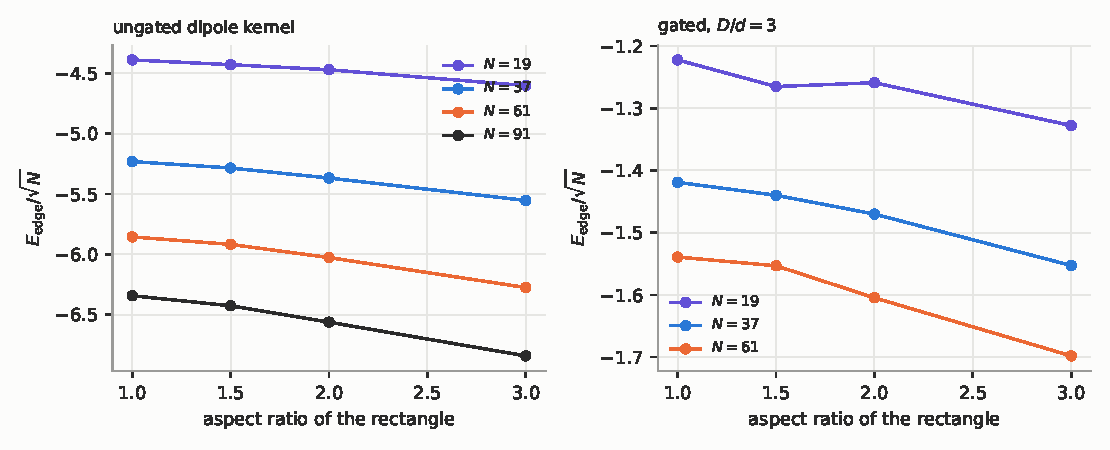
\includegraphics[width=0.92\textwidth]{figs_companion/fig_edge_aspect.pdf}
\caption{Edge energy per $\sqrt N$ against the aspect ratio of the container (best configurations; $E_{\rm edge}=E_p-Ne_{\rm lat}(\rho_0)$
with $E_p$ the \emph{penalised} energy). Monotone in the aspect ratio for the ungated kernel at all four $N$ and for g3 at $N=37,61$;
g3 at $N=19$ is non-monotone (the second point lies below the third).}\label{fig:edge}
\end{figure}

\textbf{Findings.}
\begin{itemize}[leftmargin=1.2em,itemsep=1pt]
\item \textbf{The edge excess is negative} for hard walls (a boundary particle misses neighbours), as expected for a repulsive kernel.
\item \textbf{Aspect ratio.} $E_{\rm edge}$ decreases (becomes more negative) and $E_{\rm edge}/P$, with $P$ the perimeter, increases monotonically with
aspect ratio at every $N$ for dip and at $N=37,61$ for g3; g3 at $N=19$ is non-monotone in both (registered output, reported as such). The gated ($D/d=3$) edge energy per $\sqrt N$ is smaller in magnitude by a factor of 3.4--4.0 than the ungated one at the same $N$ and shape.
\item \textbf{No clean boundary law.} Fits $E_{\rm edge}=\gamma\sqrt N+c$ have $c$ large and positive ($+15$ to $+19$ for dip) and
$E_{\rm edge}/\sqrt N$ is not constant (cover figure, panel c); with four ($N=19\ldots91$) or three points the spread of $\gamma_P=\gamma/(P/\sqrt N)$
across shapes is 12\% (dip) and 4.5\% (g3); g10 exists on three shapes only. This is a description, not a test of a perimeter law, and the verifier asked that the earlier
phrase ``holds roughly'' not be used.
\item \textbf{Defects.} Counts of interior five- and seven-fold sites are in the committed table (65 cases). Delaunay counts are
unreliable in near-square arrangements (four co-circular points); cases flagged irregular have an irregularity fraction 0.3--1.0, and
are not interpreted. A claim, made by the worker's first message, that a relaxed perfect hexagon patch lies 0.16\%, 1.2\%, 0.36\%
above the best configuration at $N=37,61,91$ was \textbf{not reproducible by the verifier and is withdrawn}; in the committed records
the lowest hexagon states at $N=37,61,91$ for the ungated kernel all contain interior defects.
\end{itemize}

\textbf{Process weaknesses (registered, not cured).} Amendments A4 and A5 (aligned starts) carry timestamps that precede their
commit; the aligned stage for $N\le37$ had already run when they were committed, and A5 was motivated by looking at success rates, and A6/A6b (extra random starts for the ungated kernel at $N=61,91$) were added after seeing
low success rates. The
Rust source was committed together with the results, not before them (the pre-registration and instrument gates were). Interior-defect
definition changed once (A1, before any count was read).

\section{A validity gate for Hugging Face and neural-network inputs}\label{sec:hf}

\textbf{Question.} Can a Hugging Face dataset or a graph-neural-network (GNN) force field supply the inputs of the gated kernel: the
electron--hole separation $d$ (hence $\tilde U(0)=4\pi d(1-d/D)$), the dielectric environment, the exciton mass and binding energy?
\textbf{Verdict: the gate fails for the two quantities that matter.}

\begin{center}\small
\begin{tabular}{@{}p{0.43\textwidth}p{0.08\textwidth}p{0.4\textwidth}@{}}
\toprule
gate & result & evidence \\ \midrule
G1 source: read-only, $<$50 MB, permissive, hashed & pass & \texttt{colabfit/JARVIS\_C2DB}, CC-BY-4.0, 1.99 MB \\
G2 2H MoSe$_2$ and WSe$_2$ monolayers present & pass & entries 3150 and 3118 identified by geometry \\
G3 any MoSe$_2$/WSe$_2$ bilayer so $d$ can be read & \textbf{fail} & no entry has two metal planes $>5$\,\AA\ apart; $\le12$ atoms \\
G4 in-plane $a$ within 2\% of $\ge2$ published values & pass & $3.3197$, $3.3190$\,\AA; largest deviation 1.13\%; agrees with PBE values~\cite{Kormanyos2015} by construction \\
G5 any excitonic/optical quantity & \textbf{fail} & only PBE energy and PBE gap \\
\bottomrule
\end{tabular}
\end{center}

The verifier re-downloaded the files (hashes identical), re-ran the extraction (byte-identical outputs) and re-read the literature
values. Corrections it required, now applied: the claim ``no Hugging Face dataset or GNN supplies $d$'' is limited to \emph{the datasets
examined} (one opened; other JARVIS 2D sets were scanned by the verifier and contain no pure MoSe$_2$/WSe$_2$ bilayer, but the report
had not shown that); the G5 gate is hard-coded to fail in the script, with the null columns in a reason string; and the machine-learned
potentials were not run. A ground-state model can in principle supply $d$ (it is a ground-state quantity), but the literature already
supplies it to about 1.5\%: metal--metal distances (the worker's reading of the figures) of 6.42--6.51~\AA\ for commensurate stackings and 7.10~\AA\ for AA
(PBE+D3~\cite{Gillen2018}, LDA~\cite{Torun2018}); the binding energies in the literature read (0.161--0.55~eV~\cite{Stier2018,Ugeda2014,Torun2018}; factor 3.4, mixing
intralayer excitons in different environments and methods with interlayer values of 0.25--0.32~eV, factor about 1.3) depend on method
and environment, which is the uncertainty an input would have to resolve and which a ground-state model cannot. Conclusion: no neural-network surrogate is warranted at this stage; a PBE value of $d$ is worth less than the
spread in $\epsilon$ and $E_b$.

\section{ETDRK4 for the driven-dissipative model}\label{sec:etd}

\textbf{What was done.} A pure-Rust radix-2 FFT with a fixed-step ETDRK4 (Cox--Matthews~\cite{CoxMatthews2002}, contour-integral
$\varphi$-functions) for the Phase~3 model, with the reservoir decay and the kinetic term in the linear part and the rate term $R|\psi|^2n_R$
in the nonlinearity; CVODE comparisons use the pinned rusty-SUNDIALS tree. Gates T-a..T-g, amendments A1--A3 dated and committed before
the runs they announce.

\begin{center}\small
\begin{tabular}{@{}p{0.2\textwidth}p{0.12\textwidth}p{0.6\textwidth}@{}}
\toprule
gate & outcome & reason \\ \midrule
T-a steady states & pass & 13/13 above threshold, worst $|n-10|/10=2.8\times10^{-13}$; 10/10 below ($|\psi|\le2\times10^{-18}$) \\
T-b order 4 & \textbf{fail} & successive ratios 2.2, 2.9, 4.5, 7.2 (registered 12--20); consistent with stiff-order reduction \\
T-c stability limit & measured & $h_{\rm first}=0.64$ at the registered point, 37$\times$ the IMEX 0.01707; $0.0034$ at $Rn_0/\gamma_R=5$ \\
T-d(i) records, $t=4000$ & \textbf{fail} for $V_0=0.5,1$ & ETD time-step error; converges to the CVODE record as $h\to0$ \\
T-d(ii) $t=16000$ & 2 of 4 pass & $V_0=0.5,1$ fail by 2--3.6$\times$ on the relative mean $n$ at $h=0.05$ \\
T-d(iii) $16\times16$ vs.\ the independent reviewer's printed digits (review of paper~I) & pass 3/3 & shifts $0.0463,0.0767,0.1065$; $n_{\rm c}=5.844,2.377,0.1000$ \\
T-e(ii) time to residual $10^{-7}$, $8\times8$ & 7.7\,s vs.\ 227\,s & factor 29 over dense CVODE, same stationarity time \\
T-f planted bugs & caught & B2 caught only by the non-stiff control \\
\bottomrule
\end{tabular}
\end{center}

\begin{figure}[ht]
\centering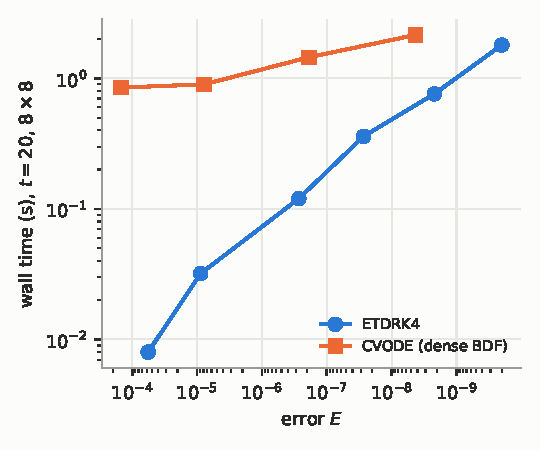
\includegraphics[width=0.52\textwidth]{figs_companion/fig_etd_wp.pdf}
\caption{Work--precision, $8\times8$ grid, $t=20$. ETD is 20--30$\times$ cheaper than dense BDF at errors $\sim10^{-5}$,
about 2.5$\times$ at $3\times10^{-9}$; no crossing was measured. CVODE wall times are the midpoints of the quoted ranges (the machine load was 4--11 on 8 cores).}
\end{figure}

\textbf{Why T-b fails.} A control with $\gamma_R$ changed at constant $n=10$ ($P=\gamma(10+\gamma_R)$) shows the step-halving error ratio rising towards 16 as
$h\gamma_R$ falls: $7.6, 10.9, 13.3, 14.6$ at $\gamma_R=20$; $19.9$ at $\gamma_R=2$ (the later ratios sit at the reference floor);
$2.2$--$7.2$ at the registered $\gamma_R=200$, i.e.\ an observed order of about 1.1--1.5 at the largest steps. Krogstad's variant
(cover panel d) has 5--15 times smaller error at $h=0.0125$ but no order 4 either. The verifier reproduced the ratios with its own ETDRK4 and a DOP853 reference ($2.25,2.90,4.49,7.21$), which excludes a
coding error. The stiff-order reduction of the Cox--Matthews scheme~\cite{HochbruckOstermann2005} is the mechanism consistent with these
data; the citation is from memory and the claim ``is exactly the stiff-order reduction'' is stronger than a single scan proves.

\textbf{Where ETD is worse than the alternatives.} (i)~Its advantage over dense BDF shrinks from 20--30$\times$ at $E\sim10^{-5}$ to about 2.5$\times$ at $3\times10^{-9}$ and the tabulated
runs do not show a crossing (at $E=2\times10^{-10}$ ETD took 1.8\,s, the same wall time as the most accurate CVODE setting, which reached
only $4\times10^{-9}$); the step count relative to CVODE grows with accuracy, so a crossing below $10^{-9}$ is a suspicion, not a measurement. (ii)~Its step limit is
not unconditional: kinetic resonances at $hw_k=2\pi n$ and, at $Rn_0/\gamma_R=5$, a limit $0.0034$, five times below the IMEX
module's. (iii)~It carries a time-step residual floor $\sim h^3$ in its stationary state (7\,$\times10^{-9}$ at $h=0.05$), so a gate with
budget $10^{-8}$ needs a smaller step. (iv)~It has no error control. The verifier's non-blocking notes: the T-d(iii) tolerances are about
the rounding of the reviewer's three-digit values (a weak consistency check); the source was committed with the results; one summary row
conflates last-stable and first-failing steps.

\section{What was not completed}\label{sec:notdone}

\begin{failbox}
\textbf{Not reported here.} (a)~The matrix-free Newton--Krylov solver (SDIRK2 with GMRES) pre-registered gates K-a..K-e were being run on
small and $64\times64$ grids when this paper was frozen; no Krylov result is claimed. (b)~The classical L6 node-arrangement study with the \texttt{rusty-Fenris-CMRR} engine and the gated kernel
had gates a, b, f and a production campaign, and is awaiting its verifier; no result is claimed, and the open-boundary study of
Section~\ref{sec:edge} is not that study. They may be reported in a later record; nothing is implied here about their outcome.
\end{failbox}

\section{Response to the external review's four improvements}\label{sec:review}

\begin{center}\small
\begin{tabular}{@{}p{0.28\textwidth}p{0.62\textwidth}@{}}
\toprule
proposal & status in this deposit \\ \midrule
Lean formalisation & done to the stated extent (Section~\ref{sec:lean}); the review's claim that Mathlib lacks Poisson summation was
checked against the pinned tree and is false for this release \\
JFNK / Krylov at $\ge64\times64$ & not complete; see Section~\ref{sec:notdone} \\
Exponential integrators & done: fails the registered order gate at the registered stiffness; useful as a fast stationary-state
solver (Section~\ref{sec:etd}) \\
L6 with Fenris-CMRR & not complete; a classical design target at most, never a prediction about excitons \\
\bottomrule
\end{tabular}
\end{center}

\section{Limitations and reproducibility}\label{sec:repro}

\textbf{Limitations.} The lattice theorem is unrefereed and AI-generated; the gated kernels are ideal grounded planes; the model
parameters of the driven-dissipative model are dimensionless and chosen for stiffness; the Wigner estimate is a harmonic criterion
calibrated on one QMC anchor; the edge study is classical, with reduced numbers of starts; the HF gate examined one dataset in depth;
the ETD tests use $8\times8$ and $16\times16$ grids and one initial seed for most gates. The pre-registered protocol L1--L6 of the
first paper is unchanged; L6 remains a classical design target.

\textbf{Files.} Lean: \url{exploration/exciton/lean/GatedKernel.lean}, \url{VERIFICATION_GatedKernel.md}. Wigner:
\url{docs/designs/EXCITON_FLUID_WIGNER_GATE.md}, \url{docs/designs/EXCITON_FLUID_WIGNER_PREREG.md}, \url{docs/designs/EXCITON_FLUID_WIGNER_REPORT.md}, \url{exploration/exciton/results/wigner/}. Edge:
\url{exploration/exciton/edge/} (\url{PREREG.md}, \url{results/analysis/cases.md}, \url{summary.json}). HF gate:
\url{exploration/exciton/hf_gate/}. ETD: \url{docs/designs/EXCITON_FLUID_ETD_PREREG.md}, \url{docs/designs/EXCITON_FLUID_ETD_RESULTS.md},
\url{exploration/exciton/rust/qf-exciton-etd/}. Response to the external review:
\url{docs/designs/EXCITON_FLUID_GATED_PEER_REVIEW_RESPONSE.md}. Figures: \url{exploration/exciton/python/companion_figures.py}.

\begin{thebibliography}{99}\small
\bibitem{CallensGated} X. Callens, \emph{Gated exciton fluids: a proof that image charges preserve complete monotonicity, a
driven-dissipative solver test on rusty-SUNDIALS, and a laboratory protocol}, Zenodo, \url{https://doi.org/10.5281/zenodo.23294615} (2026).
\bibitem{OpenAI2026} OpenAI, \emph{Universal optimality of the triangular lattice}, \url{https://github.com/openai/math}, family 090 (2026).
\bibitem{CohnKumar2007} H. Cohn and A. Kumar, J. Amer. Math. Soc. \textbf{20}, 99 (2007).
\bibitem{Astrakharchik2007} G. E. Astrakharchik, J. Boronat, I. L. Kurbakov, Yu. E. Lozovik, Phys. Rev. Lett. \textbf{98}, 060405 (2007).
\bibitem{Buechler2007} H. P. B\"uchler \emph{et al.}, Phys. Rev. Lett. \textbf{98}, 060404 (2007).
\bibitem{Boening2011} J. B\"oning, A. Filinov, M. Bonitz, arXiv:1101.1757 (2011).
\bibitem{Valenti2025} Valenti \emph{et al.}, arXiv:2501.16430 (2025).
\bibitem{Kormanyos2015} A. Korm\'anyos \emph{et al.}, 2D Mater. \textbf{2}, 022001 (2015).
\bibitem{Gillen2018} R. Gillen and J. Maultzsch, Phys. Rev. B \textbf{97}, 165306 (2018).
\bibitem{Torun2018} E. Torun \emph{et al.}, Phys. Rev. B \textbf{97}, 245427 (2018).
\bibitem{Stier2018} A. V. Stier \emph{et al.}, Phys. Rev. Lett. \textbf{120}, 057405 (2018).
\bibitem{Ugeda2014} M. M. Ugeda \emph{et al.}, Nature Mater. \textbf{13}, 1091 (2014).
\bibitem{CoxMatthews2002} S. M. Cox and P. C. Matthews, J. Comput. Phys. \textbf{176}, 430 (2002).
\bibitem{HochbruckOstermann2005} M. Hochbruck and A. Ostermann, SIAM J. Numer. Anal. \textbf{43}, 1069 (2005).
\end{thebibliography}
\end{document}
